\documentclass{article}
\usepackage[round]{natbib}
\usepackage{amsmath,amssymb,amsfonts, bbm}%
\usepackage{geometry}%
\usepackage{color}
\usepackage{graphicx}
\usepackage{authblk}
\usepackage{nameref}
\usepackage[right]{lineno}
\usepackage{subcaption}
\usepackage{tikz}
\usepackage{placeins}
\usepackage[hidelinks]{hyperref}

\newcommand{\tsinfer}[0]{\texttt{tsinfer}}
\newcommand{\kwarg}[0]{\texttt{KwARG}}
\newcommand{\argneedle}[0]{\texttt{ARG-Needle}}
\newcommand{\argweaver}[0]{\texttt{ARGweaver}}
\newcommand{\argweaverD}[0]{\texttt{ARGweaver-D}}
\newcommand{\relate}[0]{\texttt{Relate}}
\newcommand{\espalier}[0]{\texttt{Espalier}}
\newcommand{\arbores}[0]{\texttt{Arbores}}
\newcommand{\tskit}[0]{\texttt{tskit}}
\newcommand{\comment}[1]{{\it \color{orange} (#1)}}

% Bold the 'Figure #' in the caption and separate it from the title/caption with a period
% Captions will be left justified
\usepackage[aboveskip=1pt,labelfont=bf,labelsep=period,justification=raggedright,singlelinecheck=off]{caption}
\renewcommand{\figurename}{Fig}

% deal with supplementary items
\newcommand{\supplementarysection}{%
  \setcounter{figure}{0}% Reset figure counter
  \let\oldthefigure\thefigure% Capture figure numbering scheme
  \renewcommand{\thefigure}{S\oldthefigure}% Prefix figure number with S
  \section{Supplementary section}% Set supplementary section
}

% adjust inter-paragraph spacing - this one's for you, Gertjan
\setlength{\parskip}{0.5\baselineskip}

\begin{document}

\linenumbers
\title{Computing likelihoods under the SMC for a general class of ARGs.}

% First authors
\author[1, $\dagger$]{Gertjan Bisschop}

% Middle Authors
\author[2]{Alison Etheridge}
\author[3]{Peter Ralph}

% last author
\author[1]{Jerome Kelleher}
\affil[$\dagger$]{Denotes corresponding author}

\maketitle

\affil[1]{Big Data Institute, Li Ka Shing Centre for Health Information and Discovery, University of Oxford, OX3 7LF, UK}
\affil[2]{Department of Statistics, University of Oxford, OX1 3LB, UK}
\affil[3]{University of Oregon, USA}

\section{Abstract}
There currently is no way to connect the output of the diverse 
range of ARG inference methods back 
to a model that would allow us to perform a probabilistic exploration of the 
ARG space around the point estimate, or likelihood-based inference.

\section{Introduction}
\begin{itemize}
    \item ARGs are cool: There are now lots of ways to infer ARGs. Large scale either using heuristics or approximations.
    \item Models are good/essential: CwR useful but terrible for inference -> SMC
    \item Problem: we can't use models on inferred ARGs (Relate, tsinfer, ARGneedle). These methods produce point estimates. What we can't do:
        \begin{itemize}
            \item quantify uncertainty
            \item explore ARG space systematically around the point estimates. We don't have a metric on what an improvement might be.
            \item compare models of demography
            \item can't evaluate goodness of fit of model estimates
        \end{itemize}
    \item what we do here
\end{itemize}

[inspiration] great point from Wong et al.:
Note that it is important to distinguish here between structures and models: 
whether an inference method is based on 
heuristics or a rigorous mathematical model is orthogonal to the level 
of detail provided in its estimate. One could heuristically estimate a 
fully precise ARG, or statistically sample a partial, approximate ARG under 
a model such as the coalescent.

[TL;DR]: way to think about genealogies is tied to the CwR. However,
CwR does not enable us to simply compute a likelihood in the absence of a fully 
detailed history. In the past, this has given rise to approximations to the 
coalescent that had similar properties yet were significantly easier to use 
as a basis for inference. 
A similar process has taken place in ARG-based inference, 
where scalable ARG inference has been made possible due to both these approximations 
to the coalescent as well as the idea of ARGs without explicit, fully detailed 
recombination histories. What is left however is to connect the two.]

%% ARGs are awesome, or general intro about approximations

[FIX ME: introduction is very much work in progress.
start is a mess. Need to find the right way in.]
Knowledge of the exact genealogy of a set of samples would make certain problems 
in population genetics (e.g.\ inferring recombination rates) trivial.
Recent advancements in large-scale inference methods of the intricately 
interwoven paths of inheritance referred to as ancestral recombination graphs (ARGs)
\citep{rasmussen_genome-wide_2014, heine_bridging_2018, 
kelleher_inferring_2019, speidel_method_2019, rasmussen_espalier_2022, zhang_biobank-scale_2023}, 
are revolutionising the way we look at large genomic datasets.

Quite a number of studies have started to demonstrate the value of the recent ability to 
infer ARGs at scale by emphasizing the ability to rephrase many fundamental problems 
in genomics as questions on the transmission of genetic material from generation 
to generation [REFS].
Yet even though the potential of ARGs in population and statistical genetics has 
been demonstrated, the fact that these inferred ARGs lack explicit detail on 
recombination events means that it remains unclear how to connect these 
reconstructed ARGs to the stochastic/generative models that have lead us 
to study these datastructures in the first place. 

For a very long time people have assumed that what is meant by an ARG is the 
fully specified genealogical history where all events are uniquely positioned 
both in time and along the genome [Wong et al. 2023].
Yet, the ease by which such a fully detailed history can be simulated under the 
CwR, is not matched by the usability of the model for inference. 
In particular, given an ARG, there will always be an infinite amount of other 
ARGs that could have generated the observed genomic dataset 
[potentially with very different likelihoods under the CwR]
\citep{mcvean_approximating_2005}.

%% approximations have driven the rate of progress in inference
Instead, approximations of the coalescence with recombination (CwR) have  
driven our ability to perform statistical genomic inference. Two approximations 
in particular have proven to be instrumental: the sequentially Markovian coalescent, 
and its extensions (SMC) on the one hand, and the Li and Stephens model on the other. 
The impact of both models is tightly linked to the fact that they have enabled 
the reformulation of inference problems as hidden Markov models (HMM) and thus 
the use of the well-known efficient HMM-algorithms.

To improve the ability to simulate the CwR, McVean and Cardin 
provided an approximation of the CwR that is both Markovian backwards in time 
as well as left-to-right along the genome \citep{mcvean_approximating_2005}. 
By sacrificing precision on our ability to capture long range linkage 
information, the SMC became the engine of many powerful inference methods [PSMC]. 
A later improvement, the SMC', closed the gap between the SMC and the 
CwR even further.

The second key approximation is not a generative model. Rather than providing 
a mathematical description of the genealogies underlying the observed data 
the Li and Stephens or copying model pragmatically details the relationship 
of a single genome to a larger set of genomes as the result of an 
incomplete copying process \citep{li_modeling_2003}. This heuristic approach 
has been successfully applied for demographic inference [and other things: ADD] 
\citep{sheehan_estimating_2013, steinrucken_inference_2019}.

Both approaches have further formed the basis (of many) of the recent advancements in 
ARG inference methods \citep{rasmussen_genome-wide_2014, heine_bridging_2018, 
kelleher_inferring_2019, speidel_method_2019, rasmussen_espalier_2022, zhang_biobank-scale_2023}. 
A further classification of these methods could be made based on the level of detail 
that is provided on recombination events. The first real breakthrough in large-scale 
ARG inference, \argweaver, heads the first group. 
The ARGs sampled by \argweaver from the posterior distribution 
given the observed variational data, are all fully precise and detailed in the sense 
that all events are explicitly inferred. Note however that the set of possible node times 
has to be limited to enable the usage of an HMM. The other more recent methods, although 
still SMC-based, have added heuristic pre- and/or post-processing steps 
that have allowed them to extend their approach to larger sample sizes. We should also 
mention \kwarg and \texttt{ARGinfer} in this category of methods producing fully detailed ARGs 
although these are not based on the SMC or the copying algorithm. In fact they represent 
two extremes along the approximation continuum with \kwarg being entirely 
parsimony-based while \texttt{ARGinfer} is a CwR-based MCMC sampler.


%% Recent progress in ARGs through approximate structures}

The second group of methods (\tsinfer, \relate, \argneedle) has marked a significant  
leap in scalability. These methods derive their scalability at least to a certain 
degree from the fact that the ARGs they infer are approximate structures. In particular, 
recombination is an emergent property of the inferred ARGs, explaining tree topology 
changes going from one local tree to the next. The recombination events themselves 
are not explicitly inferred and are thus not part of the resulting data structure.

The computational gains from not having to pinpoint recombination events tie in 
with the inevitable uncertainty associated with ARG reconstruction [Hayman, 2022, ADD REFS]. 
Some approaches have embraced the approximate nature of the resulting ARG by, for 
example, highlighting the inability to resolve certain splits and instead representing 
them as polytomies \citep{kelleher_inferring_2019}. Taken together this means that the 
degree of completeness in which genetic inheritance from ancestors to descendants is documented 
by each of these methods varies extensively.
[TO ADD: these methods only provide point estimates]

%% The Big problem: how do you connect such approximate structures to a generative model

This has complicated the ability to connect the output of this diverse range of 
ARG inference methods to a model-based description that would allow us to perform  
probabilistic exploration of the ARG space around the point estimate, 
or likelihood-based inference.

%% what we will do
Here, the idea is to bridge this gap and use the backwards-in-time formulation of the SMC 
to compute likelihoods for for \textit{any} inferred ARG 
by integrating out the time to recombination.
The application of the SMC in a way that resonates more 
with the true direction of flow of genetic information 
results in a concrete way to formulate an algorithm 
that is \textit{general} in the sense that it can deal with the various levels of 
completeness that characterise the current state of the field of ARG reconstruction.


%%%%%%%%%%%%%%%%%%%%%%%%%%%%%%%%%%%%
\section{Methods and Results}

First, we describe in more detail what sort of information we have in estimated ARGs.
Then, we define the SMC process in a ``backwards-in-time'' way,
rather than the usual ``along-the-genome'' way.
This makes it relatively straightforward to compute the likelihood,
as we explain in the next section.
Finally, we close with a demonstration that the likelihood computation can be used
to do Bayesian inference on ancestral population sizes.

% % % % % % % % % % % % % % % % % % 
\subsection{SMC backwards-in-time}\label{par:description}

[TO DO: stress fact that this description does not add anything to McVean and Cardin although the SMC is mostly reasoned about in a left to right sense. We use the notation of McVean and Cardin here.]
In its backwards-in-time formulation, the SMC \citep{mcvean_approximating_2005} only requires a 
simple modification to the coalescent with recombination.
Instead of allowing any pair of lineages to coalesce,
the SMC is the process in which only lineage with \emph{overlapping} genomic intervals may coalesce.
Surprisingly, although this is defined in terms of a backwards-in-time Markov process,
the resulting tree-valued process along the genome is also Markov.

We now define the process more formally,
and following the notation of \citet{mcvean_approximating_2005}.
At any point in time, the state of the process is $L(t)$,
the set of labeled lineages extant at time $t$,
where each ``lineage'' is represented by a union of non-overlapping half-open intervals
which represent the ancestral material carried by that lineage,
and labels are integers.
So, we can write $L(t) = \{X_i(t)\}_{i=1}^{n(t)}$,
where the $i^\text{th}$ lineage is $X_i(t)$
and is of the form
$X_i(t) = ([x_{i0}, y_{i0}), \dotsc, [x_{im_i}, y_{im_i}))$
for some interval endpoints $x_{i0} < y_{i0} < x_{i1} < \cdot < y_{im_i}$.
The \emph{span} of this lineage is the interval $s(X_i(t)) = [x_{i0}, y_{im_i}$,
and its \emph{size} is $|X_i(t)| = y_{im_i} - x_{i0}$.
Since we look backwards in time, $t=0$ is today, and so
$L(0)$ consists of $n$ sampled lineages, labelled $0$ to $n-1$,
each represented by a single interval spanning the entire genome.
Then, the process evolves by a succession of coalescence and recombination 
events until each segment of ancestral material is only present in one lineage. 
The waiting time to next event is determined by these two competing processes 
with exponentially distributed waiting times as outlined below.

Recombination is described by a Poisson process of rate $r$ per unit of genomic length and time:
so, if $T(t) = \sum_i |X_i(t)|$ is the sum of the total sizes of all lineages,
then recombination occurs at instaneous rate $rT(t)$.
A recombination to the left of $x$ 
(i.e., between $x$ and $x-1$)
with $x>x_{i0}$ and $x<y_{im}$ splits lineage $i$ into two new lineages,
which each are given new, unique labels
(and lineage $i$ is removed).
This operation keeps the total amount of ancestral material unchanged.

Coalescence occurs between
two lineages with overlapping spans at rate $\lambda = 1/(2N_e)$
(if we assume a randomly mating, diploid population of constant size $N_e$).
The newly formed lineage acquires the union of both ordered intervals, % L is updated accordingly
and the original lineages are removed.
Although coalescence is reciprocal, here we'll define a strict total order on lineages
(see \ref{par:liks}) on all lineages in $L(t)$ based on their leftmost starting points.
For any such strict total order,
the instantaneous rate of coalescence then equals $\lambda$ multiplied by the number of overlapping pairs,
i.e., $\lambda \sum_{i \neq j} I_{ij}$,
where
\begin{equation} \label{def:coal}
I_{ij} = \begin{cases}
    1 & X_i > X_j \text{ and } s(X_i) \cap s(X_j) \neq \emptyset \\
    0 & \text{otherwise.}
\end{cases} 
\end{equation}
We say that lineage $j$ can coalesce \emph{into} lineaege $i$ if $I_{ij} = 1$
(and notice that if $I_{ij} = 1$ then $I_{ji} = 0$).

For future use, define $C_i(t)$ to be the set of lineages that can coalesce into lineage $i$,
i.e., $C_i(t) = \{X_j \in L(t) | I_{ij}(t) = 1\}$.
(Therefore, $|C_i(t)| = I_{i}(t) = \sum_{j} I_{ij}(t)$.)
Because $I_{ij}$ is defined in terms of a total order, the sets $C_i(t)$ are disjoint,
which will simplify the likelihood computations.
In particular,
although recombination affects \emph{which} lineages can coalesce into $i$,
it does not change the \emph{number} of such lineages:
in other words, a recombination event changes $C_i(t)$ but not $I_{i}$.
Another useful quantity to know is the number of lineages carrying material
at each point on the genome:
for a location $z$ and time $t$, this is
\begin{equation}
    N(t,z) = \#\{i : x \le z < y \text{ for some } [x,y) \in X_i(t) \} .
\end{equation}
Note that here we are not counting the ``gaps'' in a lineage,
so that $N(t, z)$ might be less than the number of $i$ with $z \in s(X_i(t))$.

The recombination and coalescence operations described above
either split a lineage or merge two overlapping lineages,
and so as described so far, each lineage will consist of only a single interval,
rather than a collection of intervals.
However, there is one more operation:
when a sub-segment of a lineage is ancestral to all samples,
that sub-segment is removed.
Formally, define $Z(t)$ to be the segments on which the lineages have totally coalesced:
i.e., $Z(t) = \{z : N(t,z) = 1$.
Then, each coalescence event replaces the resulting lineage $X_i(t)$
by $X_i(t) \setminus Z(t)$,
the set of intervals that results from removing $Z(t)$ from all the intervals in $X_i(t)$.

% note on the disjoint set of intervals for each lineage under the SMC
Because of this last step, a single lineage can consist of more than one disjoint interval.
As noted by \cite{mcvean_approximating_2005}, 
this implies that the backwards-in-time description of the 
SMC is slightly different from the left-to-right description,
in which single ancestors only ever span a single segment of genome.
This is depicted in fig.\ref{fig:smc-unary}:
for instance, node 8 is ancestral to all samples on the middle two trees.
However, this does not affect the distribution 
of marginal genealogies up to the roots.
More precisely, all lineages will be associated with 
a single interval up to the point where one section of the 
genome has reached its most recent common ancestor but the neighbouring parts have not.

% % % % % % % % % % % % % % % % % % 
\subsection{Estimated ARGs} \label{par:recording}

\comment{clarify what's different to McVean \& Cardin: unary nodes, maybe? and different to usual SMC stuff more generally}

Although the term Ancestral Recombination Graph (ARG) has been used to mean several things,
in the generic sense, it is a labeled graph structure that records
the inheritance of genetic material \citep{wong_general_2023}.
An ARG of the sort we consider describes the history of inheritance
of the genomic material of a focal set of individuals (that we call \emph{samples}).
Concretely, an ARG is equivalent to a collection of (non-contradictory) statements
of the form ``$c$ inherited from $p$ on the genomic segment from $\ell$ to $r$'',
where $c$ and $p$ are (haploid) genomes, and $\ell$ and $r$ are genetic coordinates.
By ``describes the history'',
we mean that each node in the ARG represents a specific (ancestral) genome,
and that the ARG specifies the genealogical tree describing how the samples are related
at each point on the genome.

% % I don't think we need the notation here:
% The process described in the previous paragraph details the transitions of the 
% set of labeled lineages $L$ through time. An Ancestral Recombination Graph 
% $\mathcal{G} = (N, E)$ capturing the various inheritance paths along the genome 
% is obtained by registering an edge represented by a tuple $(c, p, X_{cp})$ 
% whenever a lineage $c$, associated with a disjoint set of genomic intervals $X_c$, is 
% replaced by one or two lineage(s), $p$ (and $p^{\prime}$), 
% in case of a coalescence or recombination respectively.
% The last element of the tuple is the extent of the edge. It is itself a  
% disjoint set of intervals such that $X_{cp} \cup X_{cp^{\prime}} = X_c$. 
% The set of edges $E$, containing all such tuples $(c, p, X_{cp})$, 
% and $N$, the set of nodes representing all genomes in the ARG, together
% define this data structure.

So, an ARG can be thought of either as a collection of inheritance relationships
between ancestral haplotypes,
or as a sequence of genealogical trees that have common node labels.
Fig.\ref{fig:smc-unary} shows a small ARG
that describes relationships between four samples on a 100bp piece of genome,
represented as both a graph (top) and a series of local trees (bottom). 
Both structures represent the same information:
for instance, the fact that the ancestral genome at $a$
inherited the left half of its genome from ancestor 6
and the right half from ancestor 5
is seen in the fact that the first two trees have $a$ below 6,
and the remaining have $a$ below 5.
The blue dotted line from $a$ in the second tree to 5 in the third tree
draws our attention to the fact that
the path traced by $a$'s ancestry switches at that point.
In fact, $a$ is in blue because it is a \emph{recombination} node --
\comment{wait is it ``recombination node'' or ``recombinant node''?}
an ancestor that has a segment of genome inherited by a sample,
but that segment was inherited in two pieces from their parent.
Other nodes (labeled by black numbers) are either samples
or \emph{coalescence} nodes --
ancestors that are the most recent common ancestor for two samples
at some place along the genome.

Crucial for the equivalence between both representations is the presence of
nodes that only have a single child along one or more local trees --
i.e., are \emph{locally unary}.
Recombination nodes (in blue) have a single child in all trees.
However, coalescent nodes can be locally unary as well:
for instance, sample 3 inherited a longer stretch of genome from ancestor 5
than did sample 2.
In the top plot, this is visible because the pink bar below node 5
extends further to the left than does the blue bar,
while in the bottom plot, this is visible because node 5 is parent to 3
in the second tree, but not to node 2, and so is unary.

A key observation of \citet{mcvean_approximating_2005}
was that the sequence of trees along the genome
generated by the SMC was Markovian \emph{after removing all unary nodes}.
In other words, if we remove recombination nodes entirely,
and erase the unary portions of coalescent nodes,
then the distribution of the next tree can be generated only knowing the current tree.
(To see that the unary nodes makes the process non-Markov,
consider that a node in a tree might be unary either because it's about to be a coalescent node
or it already has been:
looking at the second tree, we know node 5 will be coalescent further down the sequence
because it was not present in the first tree.
So, the first tree gives us information about subsequent trees
that the second tree alone could not.)
However, removing these unary portions of nodes seems odd
when one considers the consequences in the haplotype inheritance graph
of the top figure.
As pictured, both figures tell us that
3 inherits the middle bit of the genome from 7 through 5.
However, if we erase 5 from the second tree,
does this suggest that 3 inherited a single segment from 7 along two distinct paths?
The haplotype inheritance graph above makes it clear that this is unlikely:
it is in fact reasonable to leave in these unary sections.

Furthermore, these unary nodes enable 
us to uniquely identify all lineages that were hit by a recombination event,
even if we simplify the ARG by removing all recombinant nodes
($a$, $b$, and $c$ in Fig.\ref{fig:smc-unary}). 
In the absence of these recombination nodes, a recombination can be observed 
easily enough as a change in parent going from one genomic region to the next.
Without the recombination nodes we no longer know the precise time of each recombination event,
but we do still have constraints on the time:
for instance, we know that $c$ happened somewhere between node 5 and node 7.
More generally, a recombination node must happen somewhere between the child node
and the most recent of the parent nodes.
This is again easier to visualise using the 
graph representation (blue shaded area, fig.\ref{fig:smc-unary}).
Although these unary nodes are useful and to some degree clearly inferrable,
they are not always represented by simulators or ARG reconstruction methods.
However, to our understanding this is because
the field is used to thinking in terms of the trees
rather than in terms of relationships between haplotypes,
not because of any question of knowability.
Currently, 
\argweaver{} \citep{rasmussen_genome-wide_2014} 
\tsinfer{} \citep{kelleher_inferring_2019}, and
\kwarg{} \citep{ignatieva_kwarg_2021}
estimate ARGs including unary portions of coalescence nodes.
However, it is unclear to what degree these are well-inferred,
as most evaluation of inferred ARGs thus far has focused on marginal trees
(e.g., \citet{brandt2022evaluation,kelleher_inferring_2019},
but see \citet{deng2021distribution})
and thus completely ignore such unary nodes
(and their implications for inherited haplotypes).
% ARG simplification is thus linked to the presence of unary nodes in 
% the local trees and simultaneously touches upon the question of what is 
% knowable. Many ARG reconstruction methods return a data structure that 
% is in essence a series of local trees [REFs]. 
% As highlighted, this does not need to be a contradiction. 
% All ARGs can be represented as a series of local trees \citep{wong_general_2023}.
% The important question is therefore is however about the extent by which any 
% ARG reconstruction methods incorporates the available information 
% on how nodes persist across these local trees.
% 
% [TO DO] give a good explanation (using the represented haplotypes 
% in fig. \ref{fig:smc-unary}) on why these methods can infer the extent 
% of coalescing lineages.

\comment{[TO DO]: impact of unary nodes on reasoning about the SMC in a left-to-right sense.
Is there more to say them the simple remark I made in \ref{fig:smc-unary}?}
\comment{PLR: Not that I can think of?}

In the next section we will derive an expression to compute the 
likelihood for an ARG under the SMC for which we have no information on the 
time to any of the recombination events. We will then detail an algorithm 
that allows us to efficiently compute this value by iterating over the local trees.
To do this, we will rely on the unary nodes 
to identify each lineage involved in a recombination event 
as described in this section.


\begin{figure}[!ht]
\centering
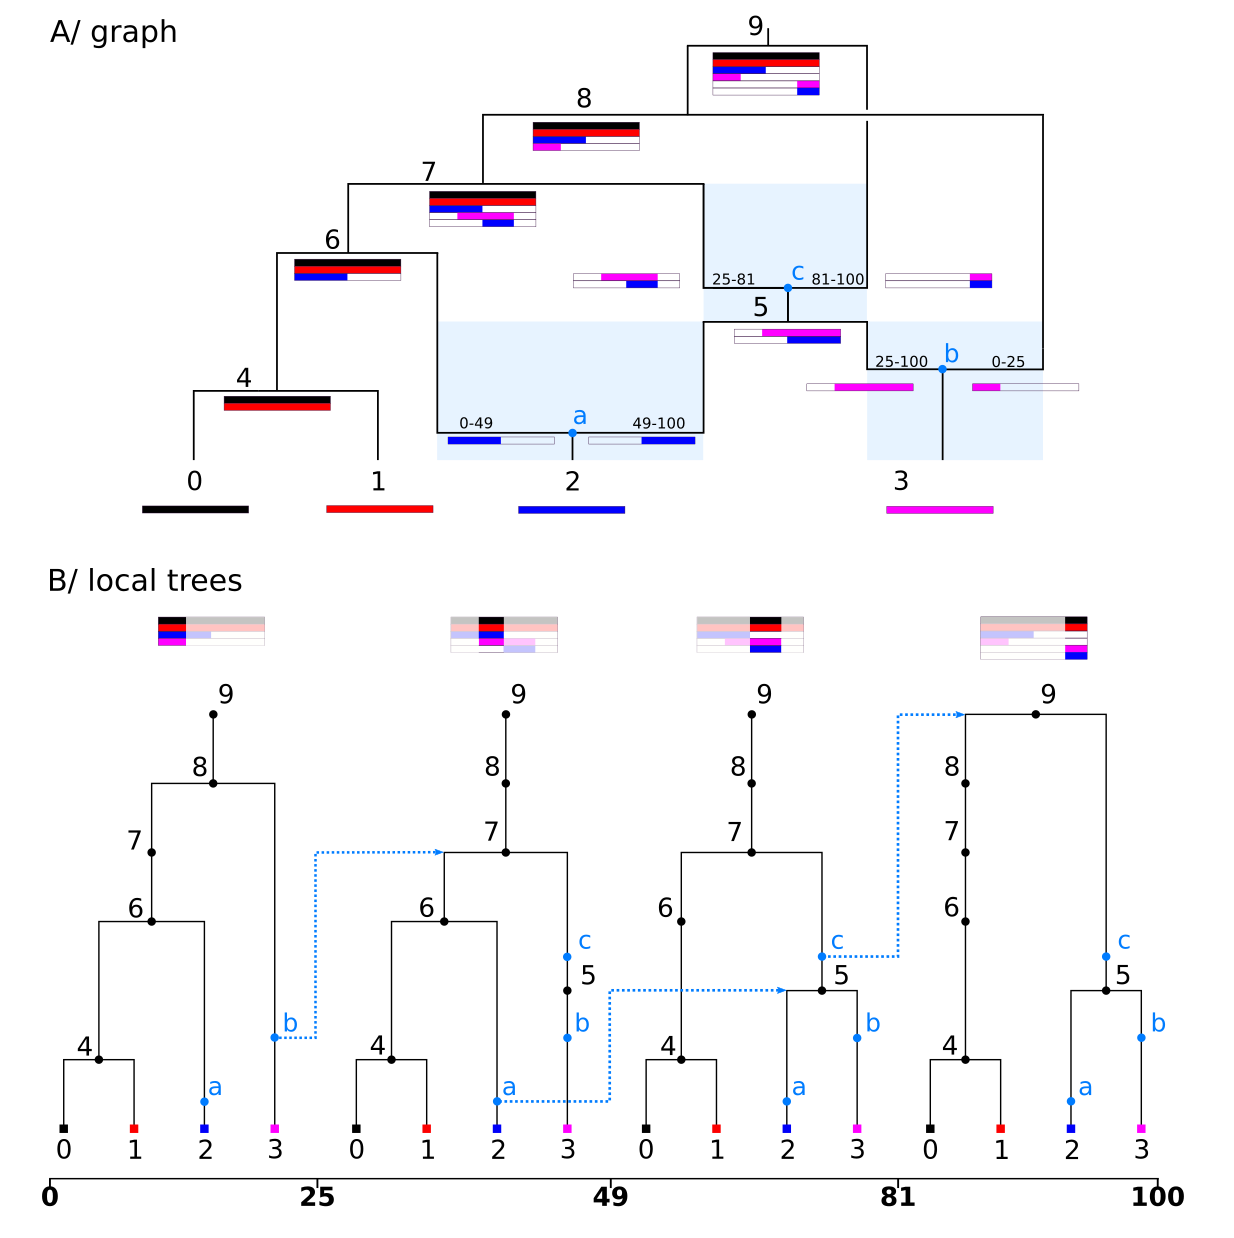
\includegraphics[width=\textwidth]{figures/smc_custom_2rows_area.png}
\caption{ARG (top) generated under the SMC and its representation as a 
series of local trees (bottom). To ensure the one-to-one correspondance 
between both representations a node is recorded for each local tree whenever 
a node is encoundered along its ancestry path in the graph representation. 
This results in nodes that (locally) have only a single child, and are therefore 
(locally) unary. Blue (unary) nodes represent recombinant nodes. 
The blue arrows shows the familiar left-to-right logic of the SMC whereby 
the floating lineage coalesces randomly
with a the remaining portion of the local tree following recombination.
Note how the presence of the unary node on a local tree is 
indicative of either a past (to the left of the local tree) 
or future (to the right) coalescence event. 
Both ARG representations can be simplified by removing the recombinant nodes. 
In that case the information we have on the time to each of these events is 
limited to the windows (blue shaded array) delimited by by the age of 
the child node $c$ associated with that lineage and the minimum age of 
the parents of the edges connecting to $c$. 
    \comment{The bits of genome that leave 5 by the left-hand path are present in 7's diagram but missing from 8's and 9's.}
 [TO DO: wanted to use the 
added in haplotype information to explain why we can actually infer the 
extent of each lineage, and thus create unary nodes in the first place.]
}
\label{fig:smc-unary}
\end{figure}



% % % % % % % % % % % % % % % % % % 
\subsection{Calculating likelihoods} \label{par:liks}

Retracing the ARG backwards in time, each coalescence event is associated with two child 
lineages, $c$ and $d$, and a single parent, $p$. By defining $C_i(t)$ asymmetrically, 
the history of each these two child lineages can be considered independently without 
risking to double count any of the coalescence events. The likelihood of 
observing the edge $(c, p, X_{cp})$ can thus be considered independently from 
the likelihood of all other edges, and in particular from the likelihood 
of $(d, p, X_{dp})$.

% extends from here means min(X_{cp})=x, max(X_{cp})=y
% improve this description here
Assuming $(c, p, X_{cp})$ extends from $x$ to $y$ along the genome and $t_i$ 
indicates the age of 
node $i$ in the ARG, then the probability of not observing a recombination across the 
entire area (span x depth) of this edge is 

% full extent of segment
\begin{equation}\label{eq:span}
A_{(c, p)}(\theta) = e^{-r (y-x)(t_p - t_{c})}
\end{equation}
% also x and y not necessarily equal to x_{c_{1}0} and y_{c_{1}m}.

What's left to compute the likelihood of the focal edge, is to take into account 
all events associated with $x$, 
the leftmost coordinate of $(c, p, X_{cp})$. 
This is either only the 
coalescence event involving 
$c$ and $d$. In that case $x=x_{c0}$ and $c$ did not coalesce until $t_p$. 
Alternatively, $x$ can be a new recombination break point that 
occurred on the lineage represented by $c$ at some time $s$ between $t_{c}$ 
and $\min(t_p, t_{p^{\prime}})$, where $p^{\prime}$ is the parent of the 
edge $(c, p^{\prime}, X_{cp^{\prime}})$ ending at $x$. The new lineage formed 
by the recombination event and starting at $x$ can be given a temporary label 
$c_s$. In both cases, the cumulative hazard of a lineage $a$ coalescing 
between time $s$ and $t$ is given by $F(c, s, t) = \int_{s}^{t} I_{c}(u)du$ 
such that:

\begin{equation}\label{eq:depth}
B_{(c, p)}(\theta) = \begin{cases}
e^{-\lambda F(c, t_c, t_p)} \lambda^{I_{cd}(t_p)} & x=x_{c0} \\
\int_{t_c}^{t_{p} \wedge t_{p^{\prime}}} r e^{-rs} e^{-\lambda F(c_s, s, t_{p})} ds \lambda^{I_{c_{s}d}(t_p)} & x=x_{c_{s}0}>x_{c0} \\
\end{cases}
\end{equation}

Here, the (second) exponential term gives the probability of not observing a 
coalescence event before $t_p$. In case of a recombination, $re^{-rs}$ further 
gives the probability of observing a recombination 
at time $s$ given a Poisson process along position $x$ with rate $r$. The 
time of the recombination is integrated out.
The last term gives the point probability density of the coalescence event 
that terminates the edge. The indicator function is used to resolve 
the non-reciprocal nature of coalescence events as defined in \ref{def:coal}.

The likelihood of ARG $\mathcal{G}$ defined by the set of edges $E$ and
given parameters $\theta$ then is

\begin{equation}\label{eq:full-lik}
\mathcal{L}(\mathcal{G}|\theta) = \prod_{(c, p) \in E} A_{(c, p)}(\theta) * B_{(c, p)}(\theta)
\end{equation}

% Does this hold for the case beyond the root of the genealogy?

[TO DO: improve this remark: when recording an ARG we do record edges in this situation,
however, msprime simulations will stop recording edges for local trees that have reached 
their local mrca.] 
Because the likelihood is computed based on edges,
and edges are no longer recorded once the local most recent common ancestor 
has been reached, we will underestimate the number of positions where 
a recombination could have occurred in case a recombination hits a 
lineage with trapped non-ancestral material (see end \ref{par:description}). 
If we assume that only a single recombination could have  
occurred, then it suffices however to provide a correction factor $g$ in equation
\ref{eq:depth}. Here $g$ represents the 
length of non-ancestral material along which a recombination would have resulted  
in the same observed local sequence of tree changes.

Note that we are only considering the topology and branch length information of any ARG. 
Extending this expression by adding the likelihood of observing a set of mutations 
given an ARG is straightforward.


\subsection{Algorithm} \label{par:algo}

\begin{figure}[!ht]
\centering
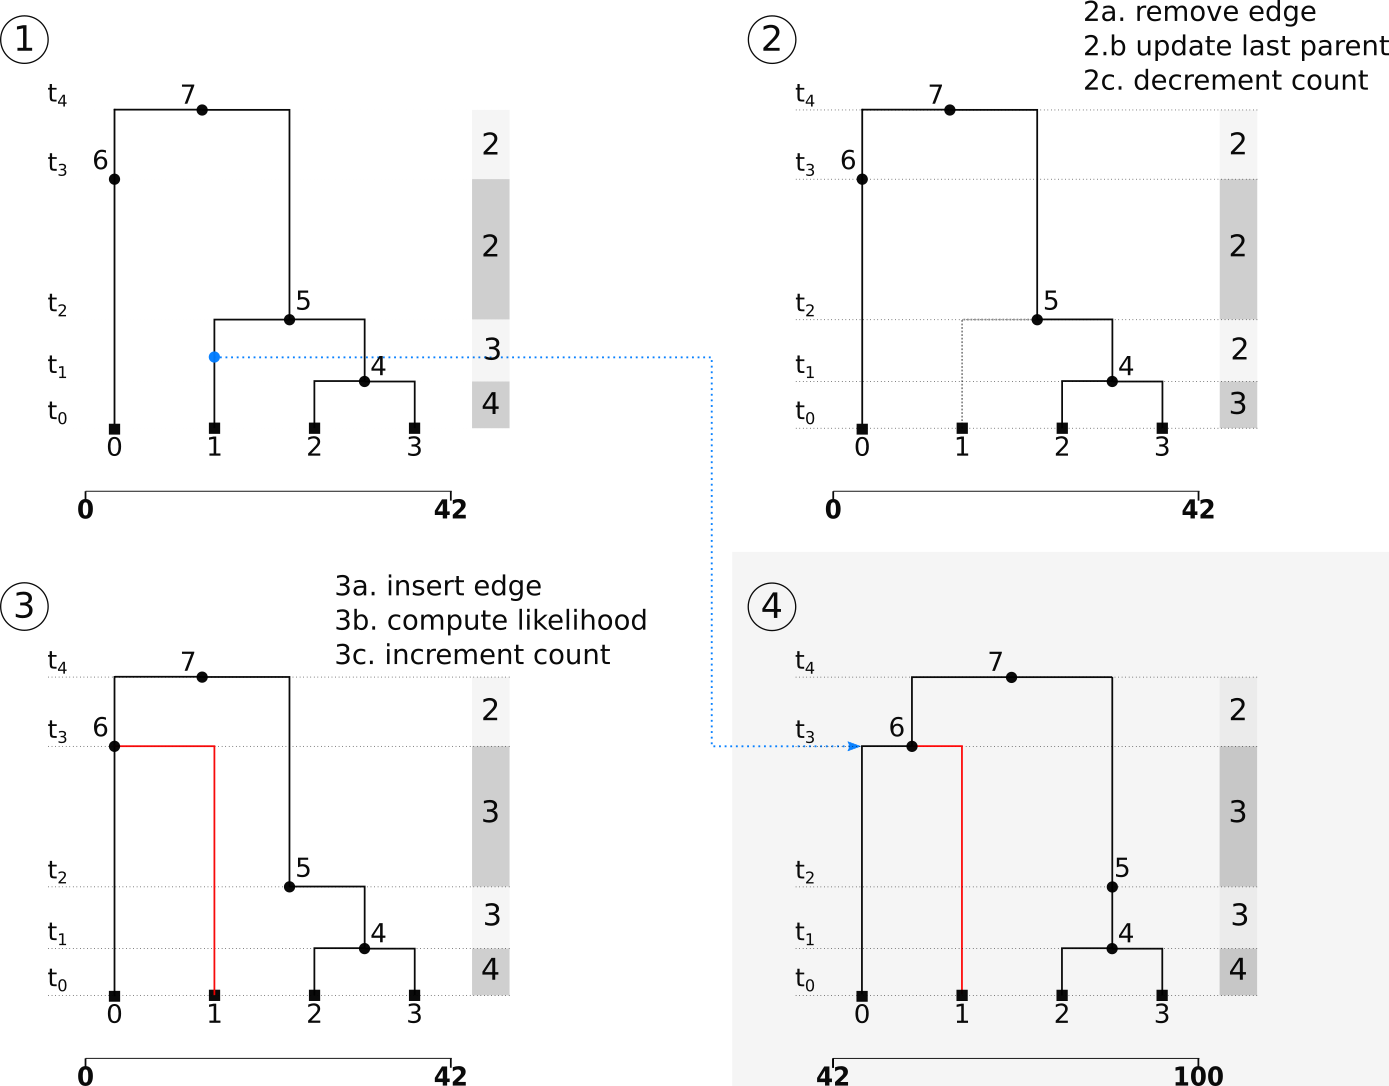
\includegraphics[width=\textwidth]{figures/ts_algo_2rows.png}
\caption{Description of algorithm: Moving along the genome we transition from  
local tree $T_1$ to the next, $T_2$ in three steps. 
Edges that do not persist in $T_2$ are 
removed first. Edges starting at the left coordinate of $T_2$ are inserted. 
After deletion or insertion of an edge the count vector $I$ is updated along the 
corresponding internode intervals. Following an insertion, and prior to updating $I$, 
the likelihood for that edge is computed as $I$ then represents the total number of 
lineages the lineage associated with this new edge can 
coalesce with. By moving along the genome in this way, each edge gets visited exactly once.}
\label{fig:algo}
\end{figure}

Although the argument outlined in the previous paragraph is valid for any ARG, here we 
will describe how to (efficiently) extract the information required to associate a
tree sequence encoding of an ARG with a likelihood under the SMC (see fig. \ref{fig:smc-unary}). 
The tree sequence format allows us to sequentially recover the local trees 
along the genome very efficiently, and in a way that allows us to reason about 
the differences between those trees \citep{kelleher_efficient_2016, ralph_efficiently_2020}. 
The order of the required edge deletions and insertions to move from one local tree $T_1$ to 
the next, $T_2$ imposes the required strict total ordering 
(see definition \ref{def:coal}) on all 
lineages in the graph needed to efficiently maintain the state of $I_e(t)$ for each focal edge $e$. 
Indeed, following the removal of edges that do not persist in $T_2$, 
we can postulate that the lineage associated with each subsequently added edge 
can only coalesce with the lineages represented by the subset of the 
visited edges that make up the (partially) reconstructed local tree $T_2$. 

This ensures we can associate a likelihood 
with all tree sequences in a single pass over all edges.
More concretely, the likelihood is computed by maintaining a single vector $I$ that tracks 
the exact number of extant lineages in each internode interval (see fig \ref{fig:algo}).
When moving from $T_1$ to $T_2$, the vector $I$ is first decremented along the internode intervals 
spanned by the time of the child and the parent of all edges that do not persist in $T_2$. 
For each subsequently inserted edge, we first compute the likelihood by computing the integral 
in eq \ref{eq:full-lik} using $I$ and then update the counts. We further keep track of 
the last parent a child node was connected to to detect recombination events.

% There is probably no need to potentially confuse people with this detail
%Remark: better to describe edges here as edge-intervals, each describing a 
%single contiguous interval of genome inheritance between a pair of nodes. 
%Under the SMC and when recording unary nodes all edges can be represented 
%by a single edge-interval.

\comment{we can probably move this to the next section} 
Note that we can accommodate for stepwise changes in the coalescence rate (or recombination rate) 
through time by intersecting the internode intervals with the rate change intervals. 
Rate changes along the genome can equally be incorporated (see \ref{sec:slicing}).

% ADD IN RESULTS
Figure \ref{sup:fig:vs-argweaver} shows the expected near-perfect correlation 
between the coalescent prior as returned by \argweaver and the likelihood as computed here. 
We simulated 1Mb of data for 10 diploid individuals 
under the SMC using human-like parameters. 100 samples were taking from the posterior every for 
a total of 1000 MCMC iterations.
 

\subsection{Slicing the ARG} \label{sec:slicing}

% slicing of the ARG
By explicitly associating a single likelihood with each edge, we can compute a likelihood 
under the SMC for any valid tree sequence. The \tskit library provides a whole range  
of subsetting operations on tree sequences allowing us to slice the ARG in time and/or space, 
as well as reduce the number of tracked samples. 
Any such subset of the tree sequence is itself a valid tree sequence 
that can again be used to compute a likelihood with. Our approach therefore strengthens 
the inherent ability of ARGs to provide us with temporal 
resolution on the inferred genealogical history of a sample. 
We can further readily incorporate changes in $N_e$ and $r$, 
both in time as well as along the genome by respectively adding intervals to $I$ 
or by splitting edges when/wherever the parameter set changes.
Figure \ref{fig:3-arg-slices} demonstrates this idea on a toy example. We simulated an ARG with 
two population size changes and subsequently estimated the posterior distribution 
using a uniform prior.

Although we rely heavily on unary nodes to provide us with the necessary 
information on recombination events, our algorithm only implicitly assumes their presence.
Without unary nodes though, our algorithm will detect a recombination event along 
both coalescing lineages in case of a (sub)tree height changes along the ARG as both 
edges would switch parent nodes. This can be mitigated by limiting the number of 
'inferrable' recombination events per coalescence event to 1 (see fig \ref{sup:fig:rec-correction}). 


%We simulated 1000 ARGs under the Hudson coalescent retaining all recombination information and computed the corresponding likelihood using \texttt{msprime} \citep{baumdicker_efficient_2021}. After removing the recombination nodes the likelihoods as defined here were computed both with and without the unary nodes. Figure \ref{sup:fig:vs-hudson} shows that the proportion of variation explained is higher when the unary nodes are retained.

\begin{figure}[!ht]
\centering
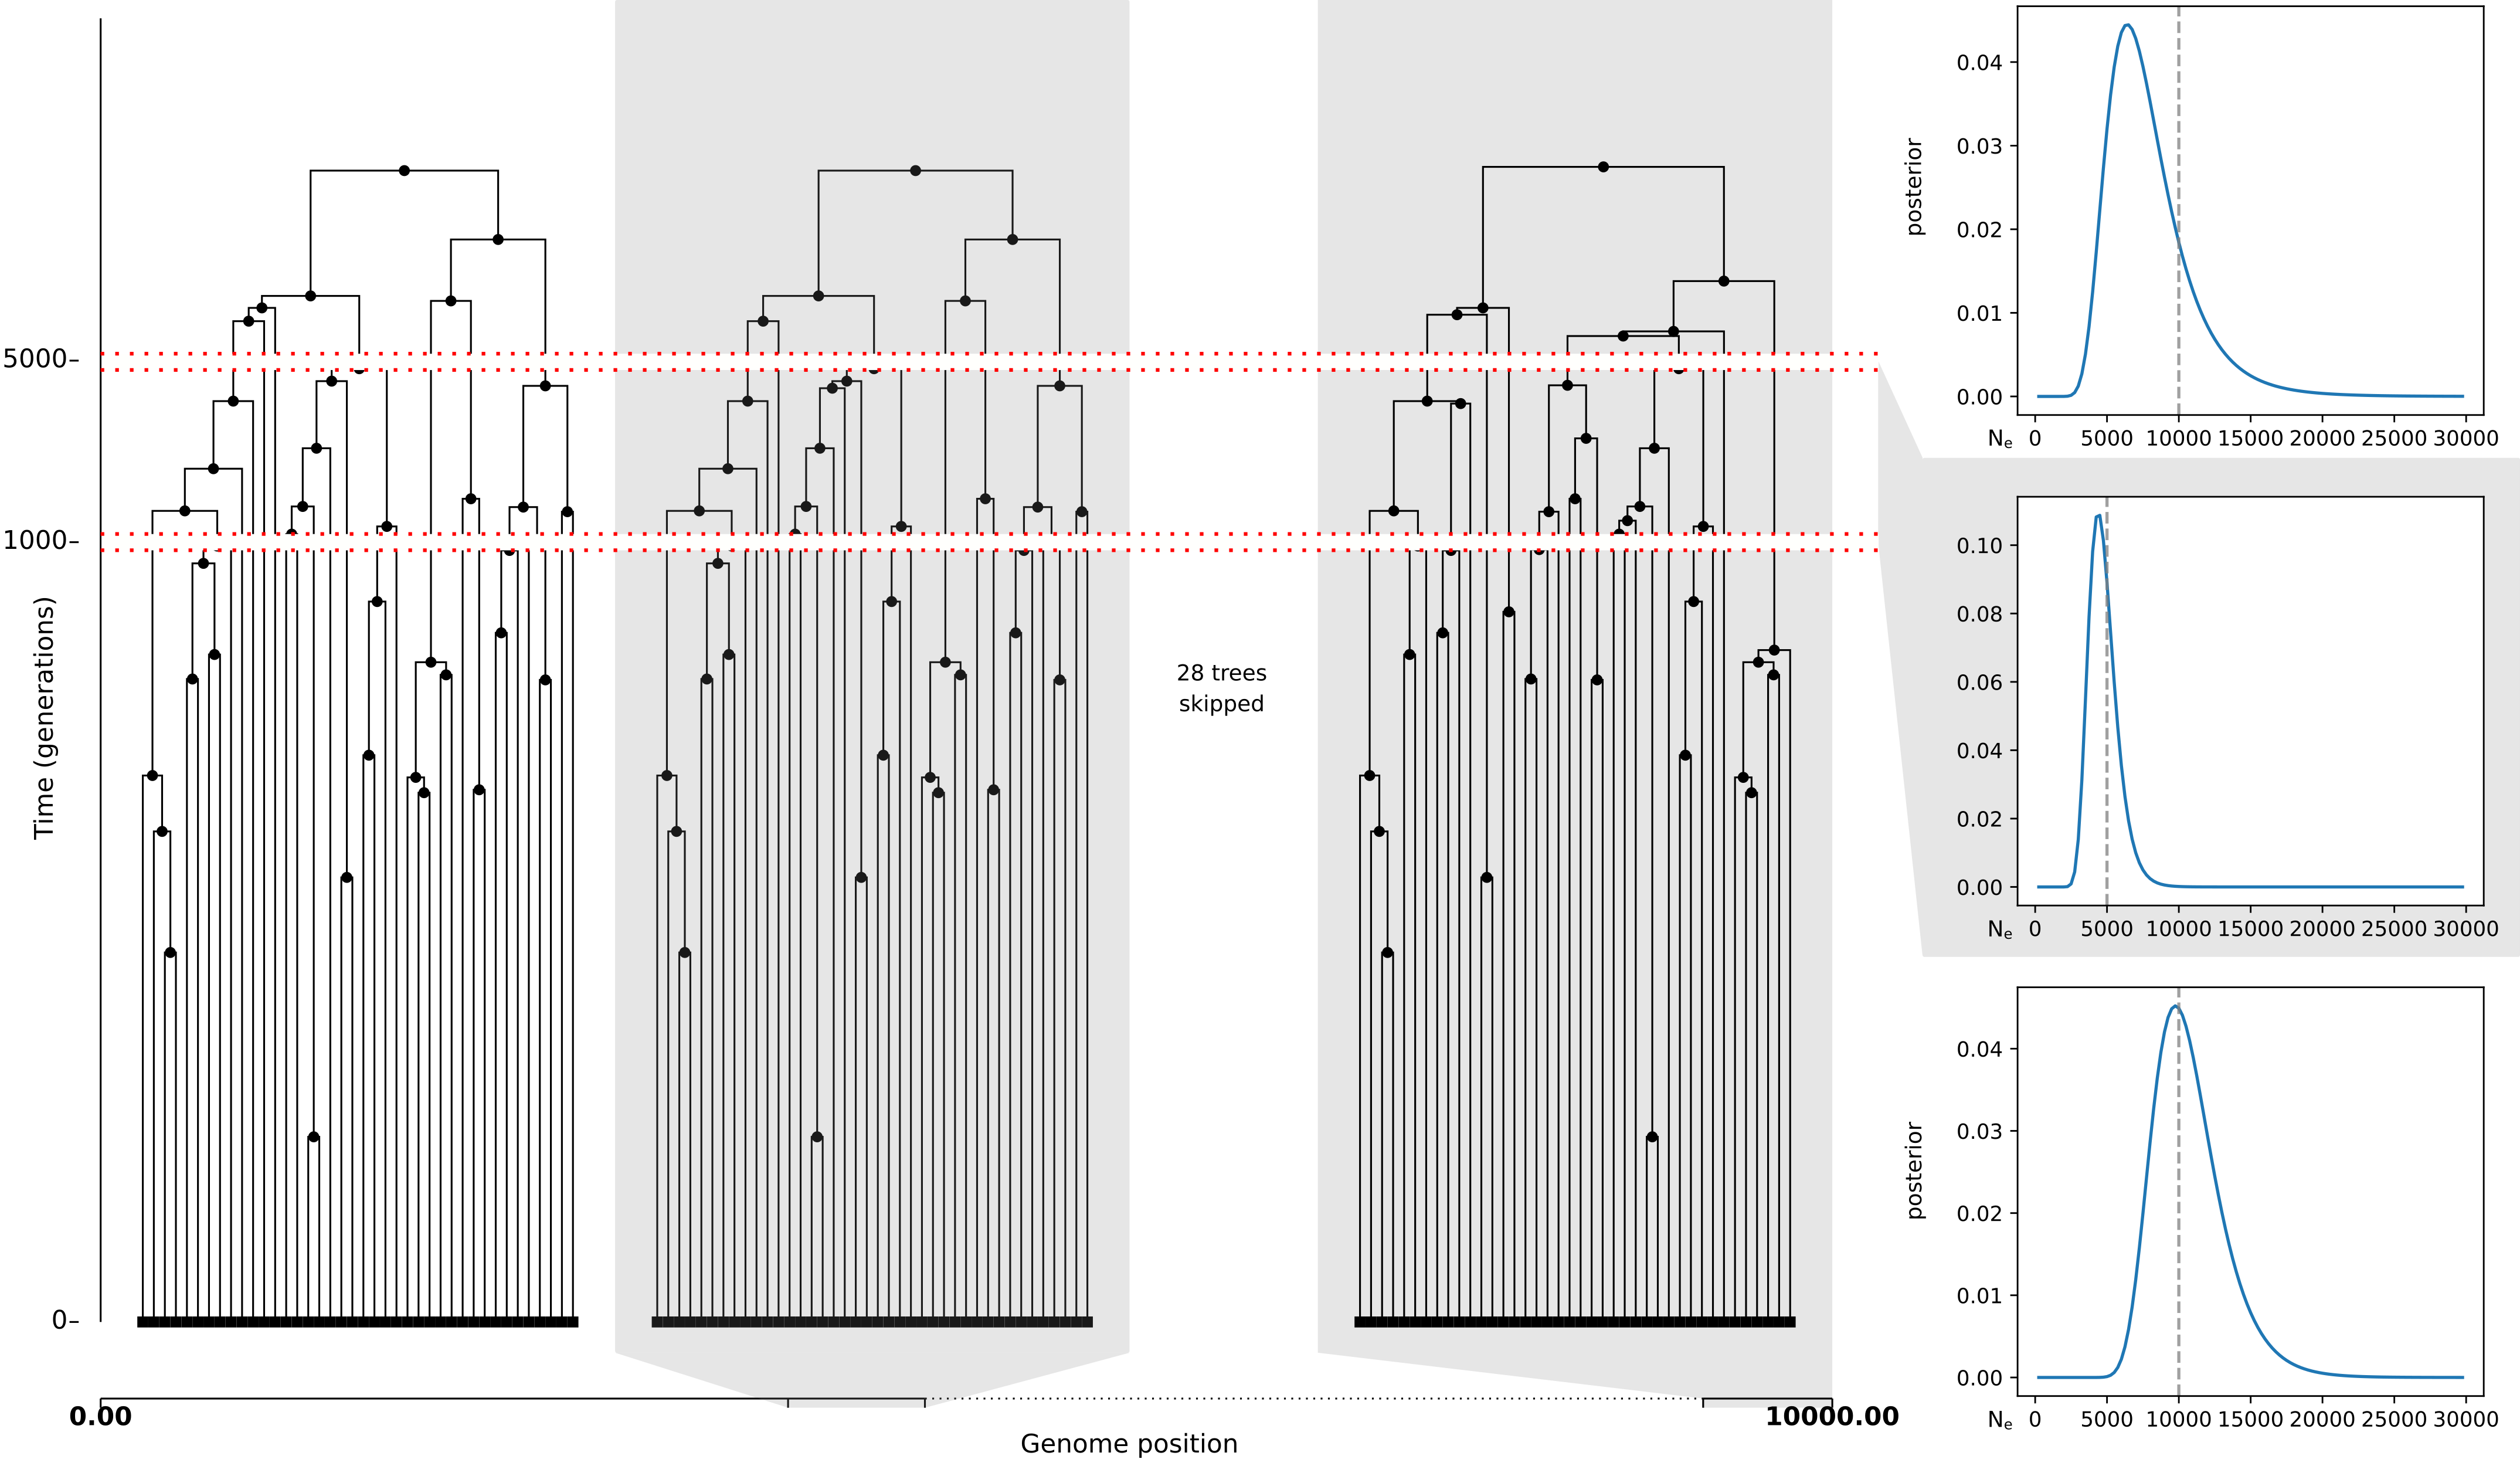
\includegraphics[width=\textwidth]{figures/3-slices-whitespace.png}
\caption{Simulated ARG under Hudson coalescent (left). $N_e$ varied was constant within each of the 3 time slices: $[(0:1000): 10 000, (1000:5000): 5000, (5000:\infty):10 000]$. Remaining parameters: L=10kb, 20 diploid samples, r=2.5e-8, 148 edges in ARG). A single $N_e$ value was estimated for each slice of the ARG as defined by the true population size change time points. The inferred posterior distribution (right) using the SMC-likelihood was obtained using a uniform prior. Number of edges per time slice: [68, 57, 23]. Locally unary nodes were omitted for clarity.}
\label{fig:3-arg-slices}
\end{figure}
 
\section{Discussion}

% a few details to be discussed
[TO DO: polytomies] The above algorithm treats each edge independently which implies 
we can deal with polytomies.
[TO DO: discuss, what if the identity of internal nodes is not preserved across trees]
[TO DO: recombination]: We do not *explicitly* assume a single recombination breakpoint to have 
occurred at each breakpoint.

Here, we have introduced a scalable algorithm to compute likelihoods 
under the SMC for a general class of ARGs. By formulating the SMC backwards in time 
we were able to associate a single likelihood value with each edge in the ARG. 
The compatibility of the algorithm with the \texttt{tskit} library allows us to 
exploit its associated efficiencies both for the current work and its future 
applications. This work will contribute significantly 
to ARG-based analysis becoming a standard part of the population 
and statistical genetics toolkit. 
In particular, we see three main applications for the work presented here. 
Firstly, the ability to associate inferred ARGs with a likelihood given a demographic 
model and an associated set of parameters, will help bridge the gap between the tremendous recent 
advances in ARG inference and the current state of the art statistical inference of 
past demography. 
Secondly, hybrid ARG-inference methods that combine the best of both 
Thirdly, inferred ARGs can be used as a good starting point for a future MCMC sampler.
heuristic and model-based inference approaches are now possible.
Finally, using a model we can quantify the uncertainty inherently associated 
with ARG-reconstruction.

% 1/ statistical inference
Currently most/all ARG-based inference methods base their analysis on marginal 
trees \citep{hejase_2022} [TO DO: add more refs]. The theory and associated algorithm 
provided here can function as a building block of [...] 
$N_e$-changes as well as multiple populations and migration can be readily incorporated 
in the current algorithm.\\


% 2/ hybrid ARG-inference: scalability + bringing ARG down from pedigree dominated phase
Hybrid backwards-in-time simulations that combine Wright-Fisher dynamics in the 
very recent past and coalescent simulations for the remaining time are a tried and tested 
approach \citep{bhaskar_distortion_2014, nelson_accounting_2020} to enable large scale 
simulations while avoiding the documented biases of the coalescent relative to the 
Wright-Fisher model \citep{bhaskar_distortion_2014, wakeley_gene_2012}. The same approach 
could be used for ARG-inference where one can rely on a heuristic inference method for 
the recent past, while using a model-based approach beyond that cutoff point.\\

% 3/ great starting point for MCMC
Any inferred ARG can be used a good starting point 
for a future MCMC-sampler. This potentially implies a massive runtime reduction by 
reducing the necessary burn-in period. Furthermore, by integrating out the exact time 
to the recombination event we further restrict the size of the ARG space that needs to 
be explored. This MCMC-sampler would again rely on the tree sequence data structure to 
efficiently generate and evaluate any new proposal (see \citep{mahmoudi_bayesian_2022}).

% 4/ quantifying uncertainty [unfinished]:
Acknowledging the uncertainty associated with ARG inference does not 
necessarily require a full-blown MCMC sampler. Instead, recognising those parts of 
the ARG for which we lack information for confident reconstruction and resolving 
them stochastically by sampling from the coalescent rather than completely arbitrarily 
would already be a major step forward.
Furthermore, quantifying uncertainty would not necessarily always have to be associated 
with sampling from subset of all compatible genealogies. Uncertainty could also 
be quantified and passed on as metadata to the nodes in the data format storing the ARG.
% can something similar be done for stacked recombinations?

As a final remark, the described algorithm relies heavily on the presence of locally unary 
nodes in the tree sequence to correctly identify the full extent of all lineages going back 
through time. Although their presence is crucial to our ability embed any local tree in the 
ARG, the concept and their importance are still relatively new (but see 
\citet{wong_general_2023}). Although we have briefly touched upon the observation that in 
the presence of unary nodes we seem to augment the left-to-right logic of the SMC 
with some additional information. 
We believe that the topic of locally unary nodes in general requires further exploration. 
And more specifically, we see it as future work to fully quantify to what extent the 
absence of these locally unary nodes will affect the shape of the likelihood surface given 
any set of parameters.\\

[ TO DO final conclusion?]


\section{Data availability}

All scripts and data used for this manuscript are available on https://github.com/gertjanbisschop/smc-bit-paper
An implementation of the algorithm is available on https://github.com/gertjanbisschop/runsmc.
\FloatBarrier
\bibliographystyle{plainnat}
\bibliography{refs.bib,paper.bib}

\pagebreak 

\supplementarysection
\section*{Supplementary Information}


\begin{figure}[!ht]
\centering
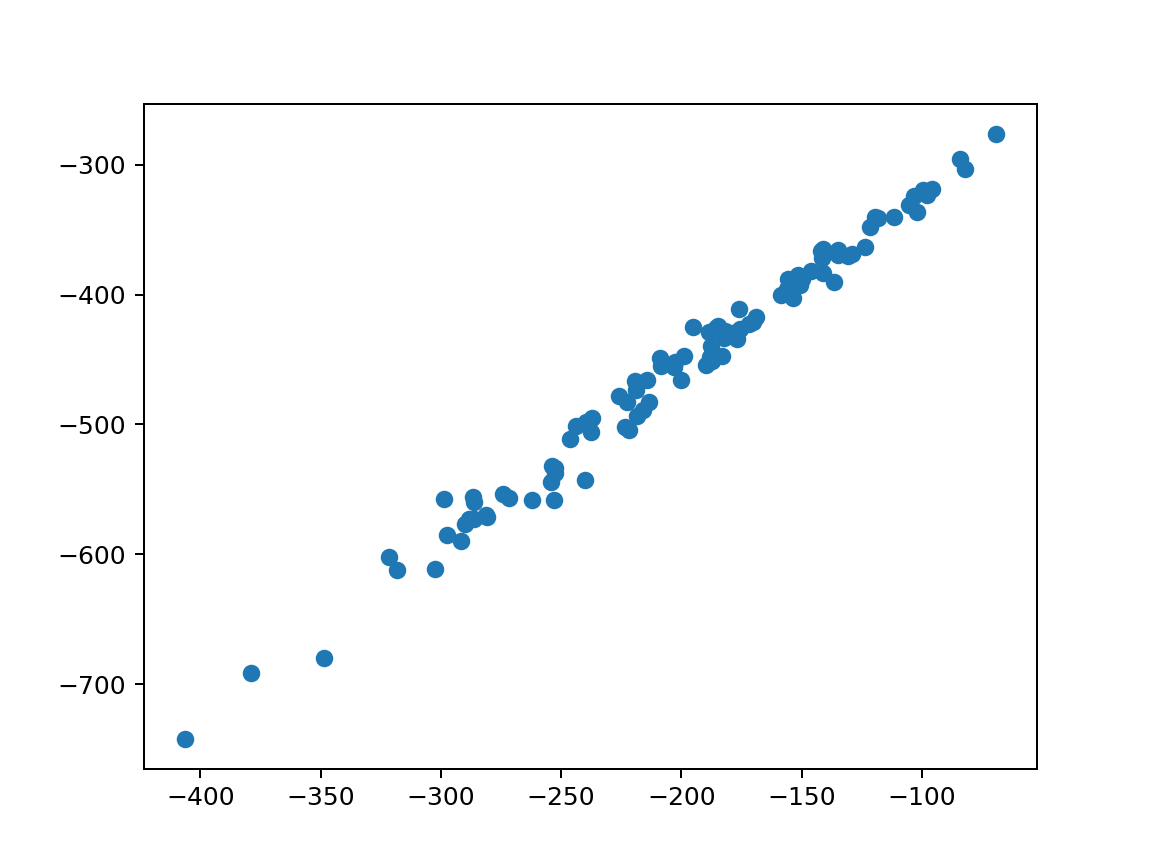
\includegraphics[width=0.75\textwidth]{figures/supplementary-figs/argweaver_vs_runsmc.png}
\caption{Simulated 10kb sequence under human-like parameters, 10 diploid samples. Inferred ARG using ARGweaver. Scatterplot is comparison of prior (discretized SMC) as reported by ARGweaver (x-axis) and likelihood as defined here (y-axis).}
 \label{sup:fig:vs-argweaver}
\end{figure}


\begin{figure}[!ht]
\centering
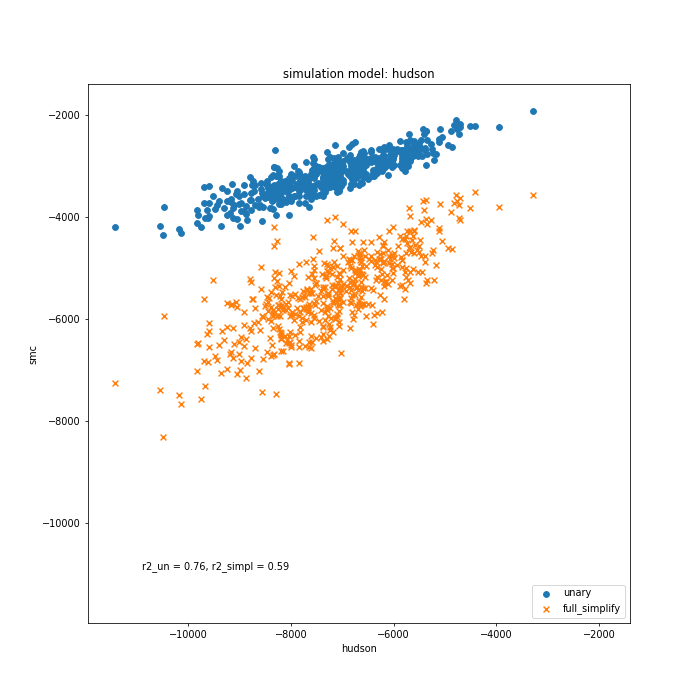
\includegraphics[width=0.75\textwidth]{figures/supplementary-figs/v_hudson_unary_simpl.png}
\caption{Compare likelihoods Hudson (full ARG) and SMC with and without unary nodes (without recombination nodes): placeholder for final figure with similar content.}
\label{sup:fig:vs-hudson}
\end{figure}


\begin{figure}[!ht]
\centering
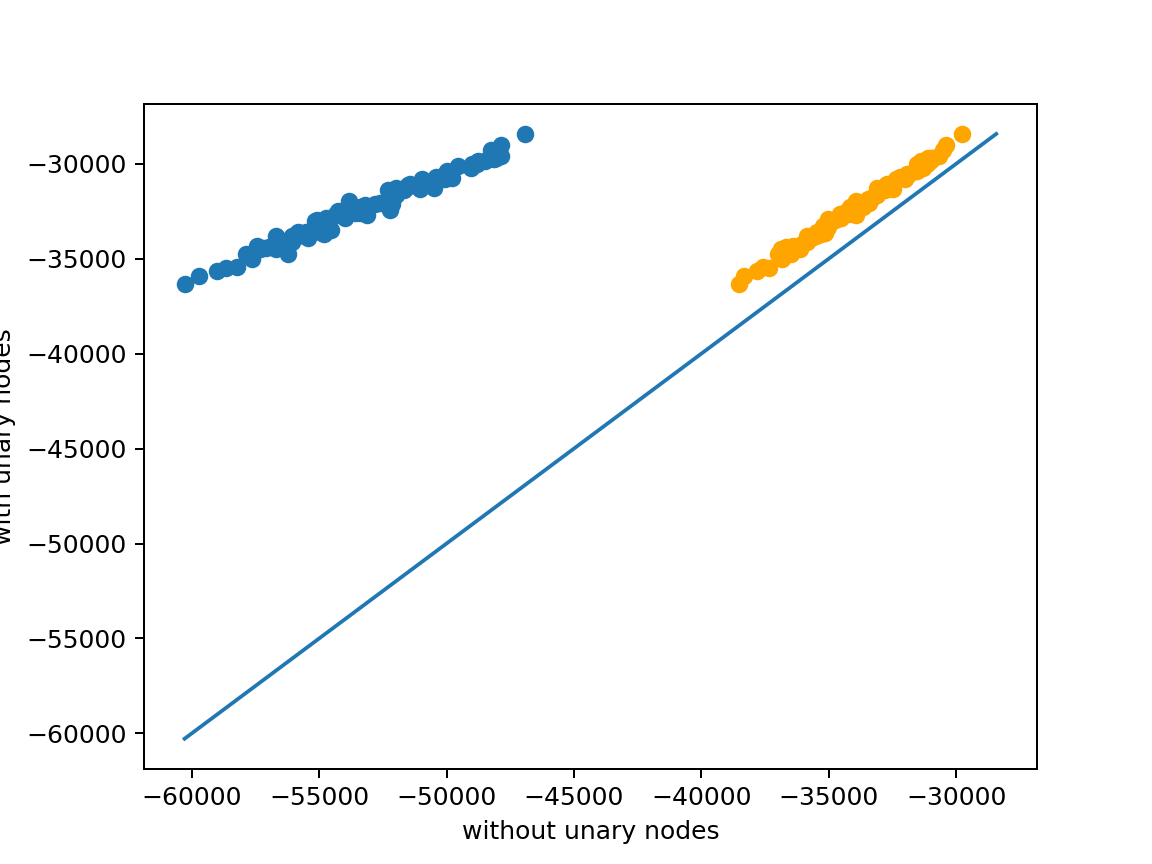
\includegraphics[width=0.75\textwidth]{figures/supplementary-figs/without_unary.png}
\caption{Simulated 1Mb of sequence under human-like parameters. Computed likelihood as defined here with unary nodes (y-axis), and without, blue dots (x-axis). By limiting the number of recombinations (to 1 event) leading up to a single coalescent node we obtain the values in orange.}
 \label{sup:fig:rec-correction}
\end{figure}

\begin{figure}[!ht]
\centering
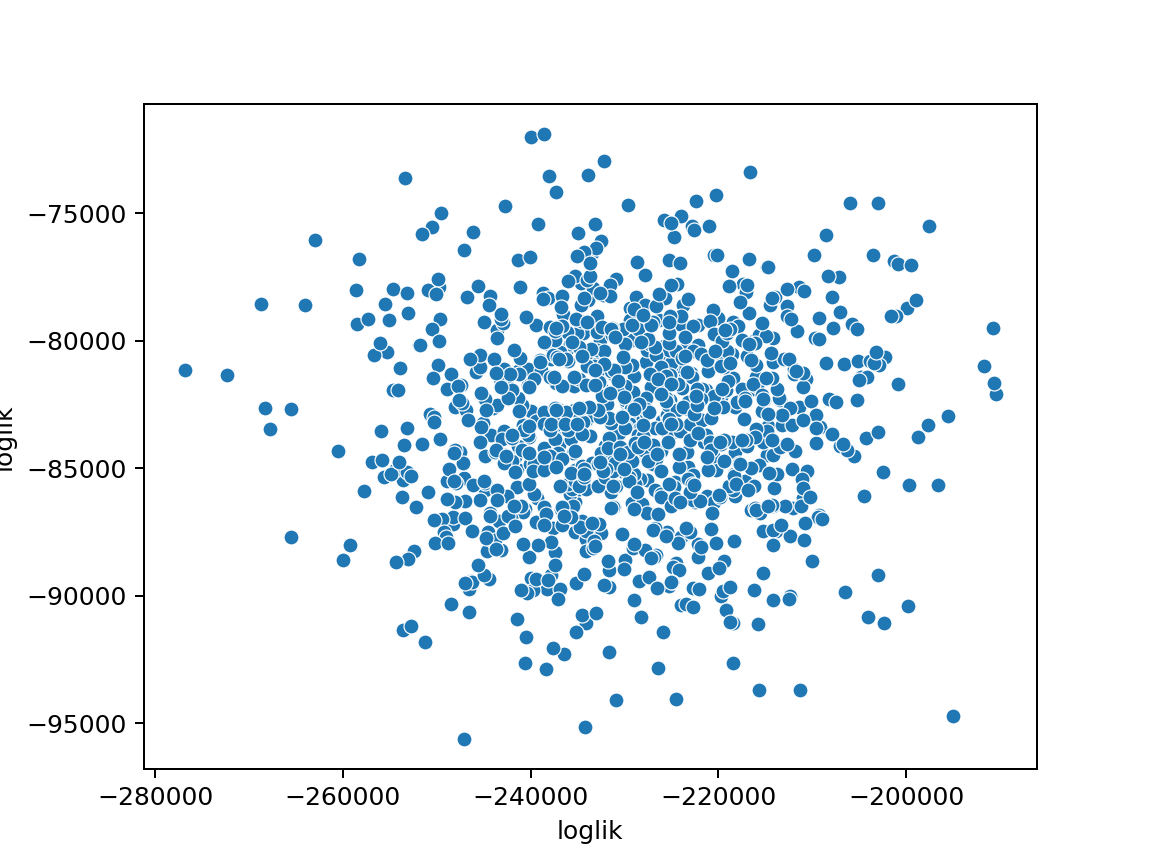
\includegraphics[width=0.75\textwidth]{figures/supplementary-figs/hudson_liks_vs_tsinfer_smc.png}
\caption{Simulated full ARG for 1Mb sequence under human-like parameters (100 diploid samples). Computed likelihood (x-axis) under Hudson. Then inferred ARG with \tsinfer following a random sprinkling of mutations and computed likelihood under SMC (y-axis)}
 \label{sup:fig:hudson-smc}
\end{figure}

\begin{figure}[!ht]
\centering
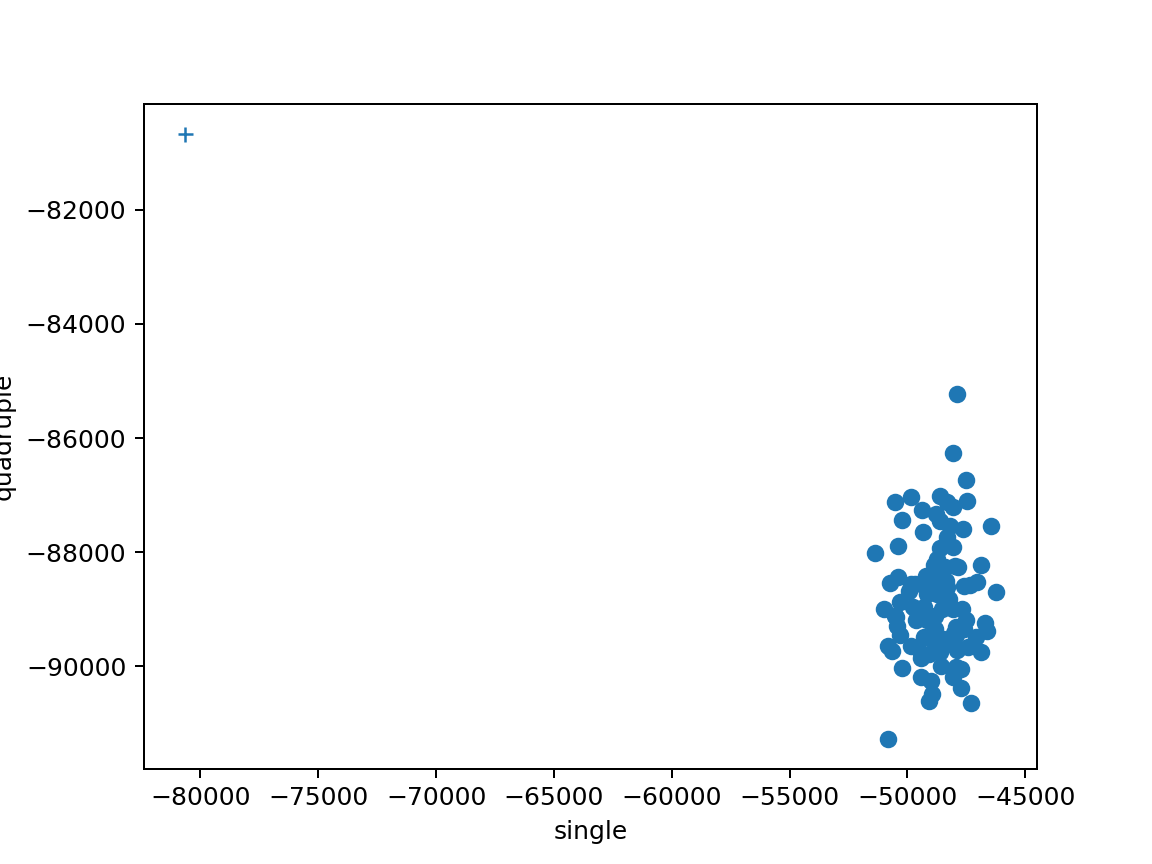
\includegraphics[width=0.75\textwidth]{figures/supplementary-figs/single_rep_human_like_1gb.png}
\caption{Single replicate from the dataset simulated above with a 100 random sprinklings of mutations. Likelihood under the SMC, mutation rate $\mu=1.25e-8$ (x-axis), and with mutation rate $4*\mu$ (y-axis). Likelihood for the full ARG under Hudson is indicated with the cross.}
 \label{sup:fig:single-tsinfer}
\end{figure}

\end{document}
